\label{unit1}
% A review of the MultiSeq main window
% Go over the shortcuts and so forth
% We should create an in-depth image with indicators of what is what

\section{The MultiSeq Graphical Environment}
MultiSeq is accessed as an extension within VMD.  To begin MultiSeq,
launch VMD and:
\begin{enumerate}
\item In the VMD main window, click on the \textsf{Extensions} Menu.
\item In Extensions, select \textsf{Analysis} $\rightarrow$
\textsf{MultiSeq}.
\end{enumerate}
(alternatively, if you are a fan of command lines, you can type
`\texttt{multiseq}' into the VMD terminal window)

The main MultiSeq window (see Fig.~\ref{fig:main}) will appear (note
that the first time you run MultiSeq, you will be prompted to download
necessary databases before seeing the main window).

\begin{figure}[here]
 \centerline{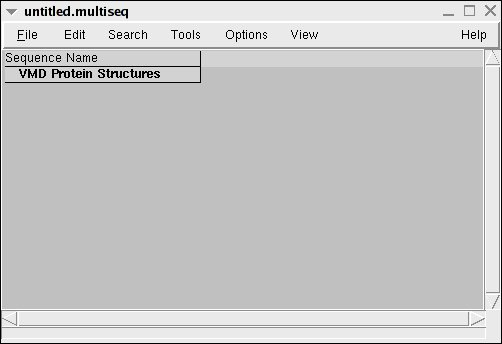
\includegraphics [width=5in]{./pictures/main_window.jpg}}
 \caption{Main MultiSeq Window With No Structures Loaded}%more information in caption about views etc.
\label{fig:main}
\end{figure}

%\subsection{MultiSeq Window Shortcuts}
%The main MultiSeq window has several shortcuts that provide complementary information with 
%additional functionality for the analysis of alignments.  For the purposes of examining these shortcuts, we will 
%use several structure and sequence files of the catalytic domain of AARSs.  
% The image with shortcut indicators will be around here
